\chapter[Experiment]{Experiment result} \label{c:tc2} 

\section{Cross correlation}

\begin{figure}[H]
\centerline{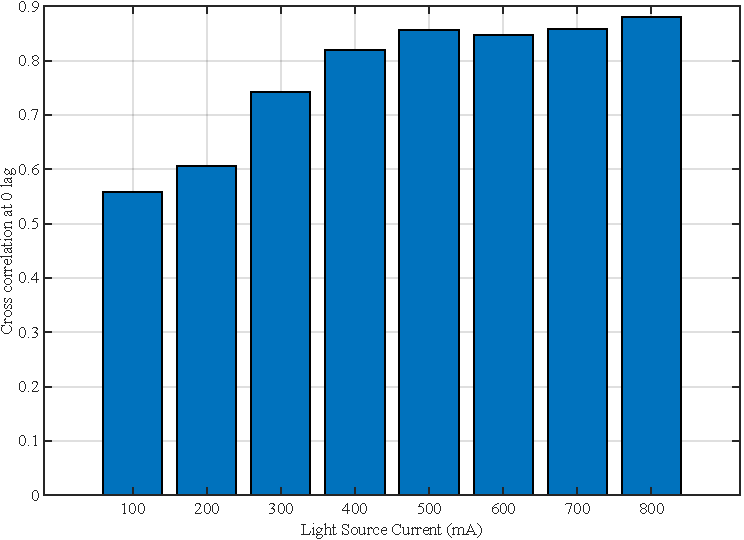
\includegraphics[scale=1]{5-Experiment/Cross correlation.pdf}}
\caption{Cross correlation of active optrode and inactive optrode channel at different light source power with no input signal at the active optrode}
\label{fig_Cross correlation}
\end{figure}

For the digital signal processing algorithm to work correctly, the noise in the two light channels must be highly correlated.  By directly taking measurements from the two receiver channels without any processing algorithm, with the light source turned on and no input to the optrodes, we can calculate the cross-correlation between the channels as shown in Fig.~\ref{fig_Cross correlation}.  At low light source power, the noise of the light receiver board dominates the noise from the light source.  The nerve signal and light source noise increase proportionally to the increase of light power, while the light receiver board noise stays the same.  When the light source current exceeds \qty{500}{\mA}, the light source noise dominates the whole noise in the system, and the normalised cross-correlation remains constant at $\sim$0.8, suggesting the possibility of active noise cancelling.

\section{Noise comparison}


\begin{figure}
\centering
\begin{subfigure}{1\textwidth}
  \centering
  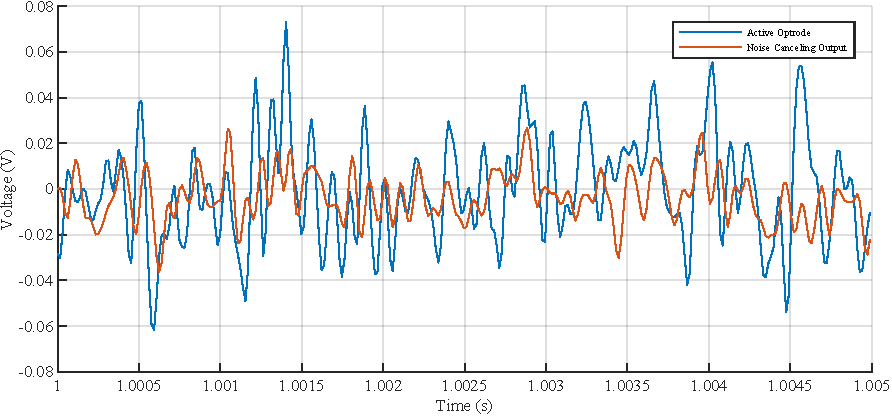
\includegraphics[scale = 0.8]{5-Experiment/500mA Signal_a.pdf}
  \caption{}
  \label{fig_500mA Signal_a}
\end{subfigure}
\begin{subfigure}{1\textwidth}
  \centering
  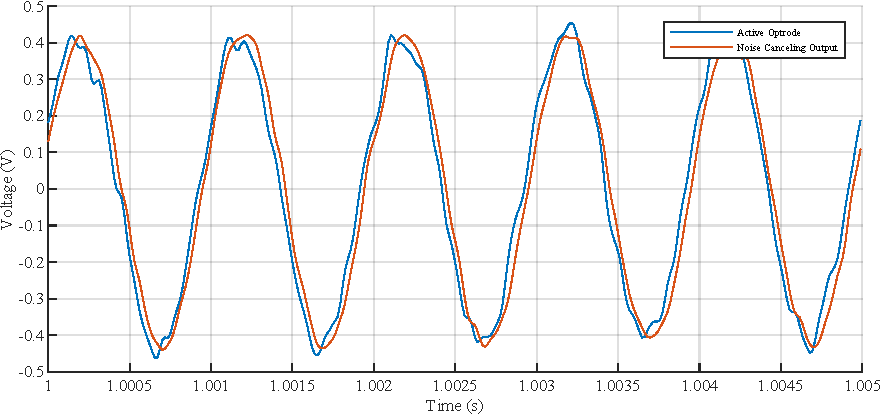
\includegraphics[scale = 0.8 ]{5-Experiment/500mA Signal_b.pdf}
  \caption{}
  \label{fig_500mA Signal_b}
\end{subfigure}
\begin{subfigure}{1\textwidth}
  \centering
  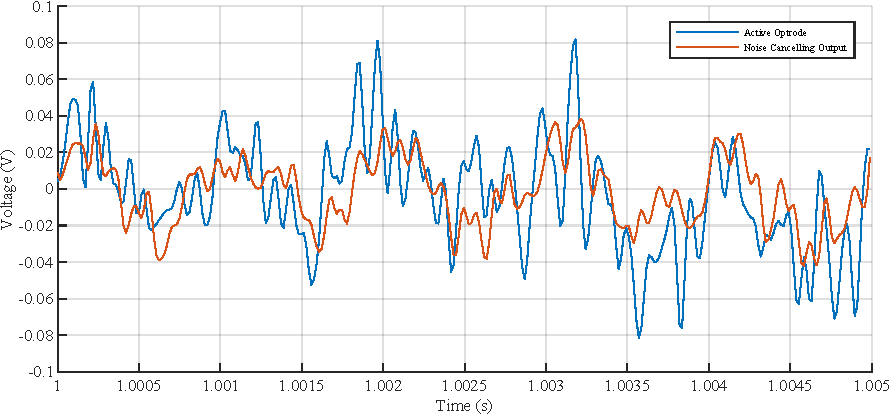
\includegraphics[scale = 0.8 ]{5-Experiment/500mA Signal_c.pdf}
  \caption{}
  \label{fig_500mA Signal_c}
\end{subfigure}
\caption{(a) \qty{500}{\mA} light source current with zero input signal at the active optrode (b) \qty{500}{\mA} light source current with \qty{200}{\mV} peak to peak \qty{1}{\kHz} sinusoidal input signal at the active optrode (c) \qty{500}{\mA} light source current with \qty{10}{\mV} peak to peak \qty{1}{\kHz} sinusoidal input signal at the active optrode}
\label{fig_500mA Signal}
\end{figure}

Fig.~\ref{fig_500mA Signal_a} shows the captured, digitised signals before (``Active Optrode'') and after (``Noise-Cancelling Output'') the noise cancelling process is applied when the optrode input is shorted.  The Active Optrode channel clearly has a substantially larger amplitude than the Noise Cancelling Output channel.  However, these two signals still have a normalised cross-correlation of 0.4, implying there is still room to improve the performance. In fig.~\ref{fig_500mA Signal_b}, a large \qty{200}{mV} sinusoidal signal is applied to the optrode.  Again, the Noise Cancelling Output channel has substantially less noise than the Active Optrode channel, confirming that the algorithm is working in the case of sinusoidal signals, even when these are much larger than the noise level.  Fig.~\ref{fig_500mA Signal_c} shows a small \qty{10}{mV} sinusoidal signal applid to the optrode.  The blue active optrode channel looks like a ramdon signal with some high frequency noise, while the red noise cancelling output channel shows a clear periodic signal at \qty{1}{kHz}.  Although the noise cancelling output channel still has a lot of high frequency noise, it shows the ability to recover small amplitude signals from noisy active optrode channel.

Fig.~\ref{fig_RMS value for ch1 and DSP output} shows the comparison between the root mean square (RMS) value for the Active Optrode channel and the Noise Cancelling Output channel for different light source currents when no voltage is applied on the optrode.  The RMS value of the Active Optrode channel (blue bars) raises when the light source current is increased showing an approximate linear relationship between the noise in the channel and the light source drive current. Similarly, the red bars show the RMS value of the Noise Cancelling Output channel. 

\begin{figure}[h]
\centerline{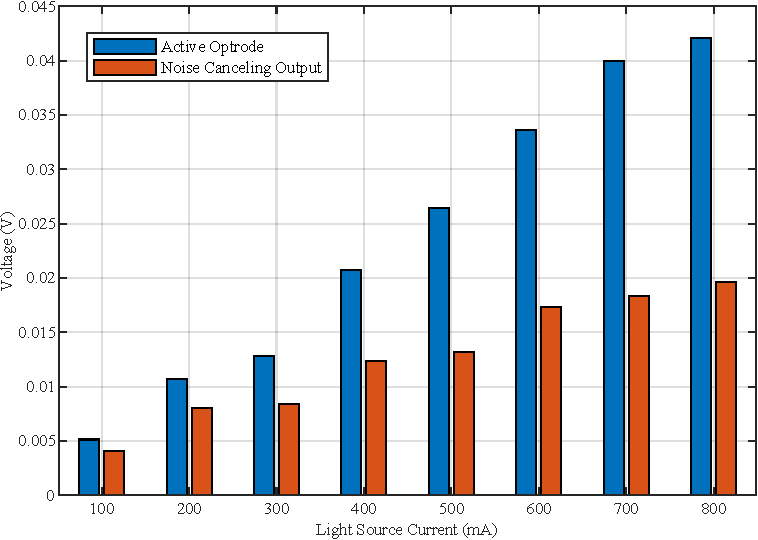
\includegraphics[scale=1]{5-Experiment/RMS value for ch1 and DSP output.pdf}}
\caption{Output Root-Mean-Square at different light source current with zero input signal at the active optrode}
\label{fig_RMS value for ch1 and DSP output}
\end{figure}

We can see that, at lower light source currents, the noise reduction seen in the Noise Cancelling Output channel is modest.  As the light source current increases, the noise in the Noise Cancelling Output channel grows slower than that in the Active Optrode channel, improving the relative noise reduction (i.e. the ratio between the two channels) with increasing light intensity.  The relative noise reduction plateaus at about 50\,\% noise reduction when the light source current is above \qty{500}{mA}, matching the cross-correlation result above.  Since the signal received from the optrode is ideally proportional to the light intensity (or light source drive current), we will see that the signal-to-noise ratio improvement the proposed system achieves is better at higher light source drive currents. 

\section{Optical input test with sinusoidal signal}

\begin{figure}[H]
\centerline{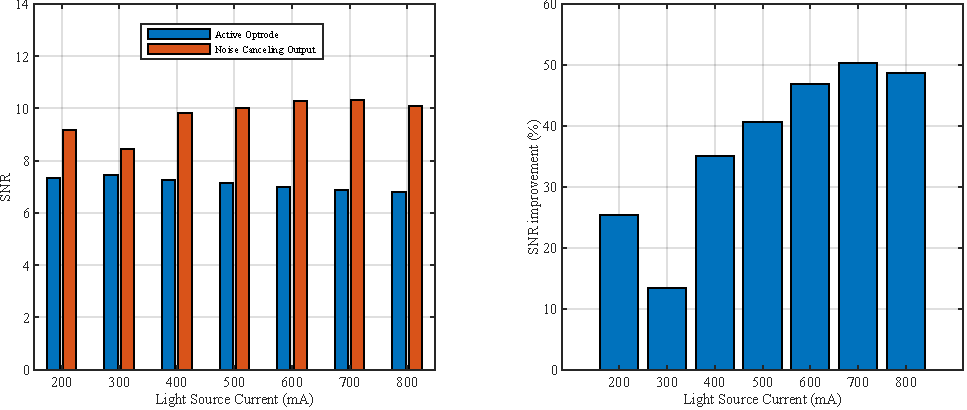
\includegraphics[width=1\linewidth]{5-Experiment/SNR (200mV input).pdf}}
\caption{(a) Signal-to-Noise-Ratio at different light source current with \qty{200}{\mV} peak to peak \qty{1}{\kHz} sinusoidal input signal at the active optrode (b) SNR improvement at same condition}
\label{fig_SNR (200mV input)}
\end{figure}

\begin{figure}[H]
\centerline{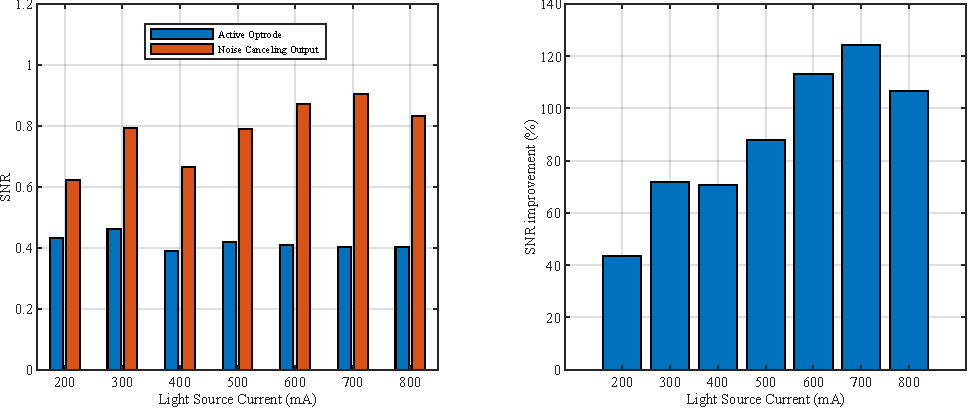
\includegraphics[width=1\linewidth]{5-Experiment/SNR (10mV input).pdf}}
\caption{(a) Signal-to-Noise-Ratio at different light source current with \qty{10}{\mV} peak to peak \qty{1}{\kHz} sinusoidal input signal at the active optrode (b) SNR improvement at same condition}
\label{fig_SNR (10mV input)}
\end{figure}

Fig.~\ref{fig_SNR (200mV input)} and fig.~\ref{fig_SNR (10mV input)} show the signal-to-noise ratio and signal-to-noise ratio improvement before and after the active noise cancelling process, for \qty{200}{mV} and \qty{10}{mV} sinusoidal inputs applied to the optrode, at different light source currents.  There is an outlying data point at the \qty{300}{mA} light source current, but overall the data matches the previous result that (i) at lower light source currents the signal-to-noise ratio improvement is modest, (ii) as the light source current increases, the signal-to-noise ratio improvement increases and (iii) as the light source drive current exceeds \qty{500}{mA}, the signal-to-noise ratio improvement plateaus. The power spectral density plots in Fig.~\ref{fig_Periodogram 500mA (10mV input)} shows a comparison of the Active Optrode channel (a) and Noise Cancelling Output channel (b) at \qty{500}{mA} light current with a \qty{10}{\mV}, \qty{1}{\kHz} sinusoidal signal applied at the active optrode.  The \qty{1}{\kHz} signal level in both graphs stays the same, while the noise floor magnitude drops by \qty{5}{dB} to \qty{10}{dB} in the Noise cancelling Output channel, matching the results from previous readings.

\begin{figure}[H]
\centerline{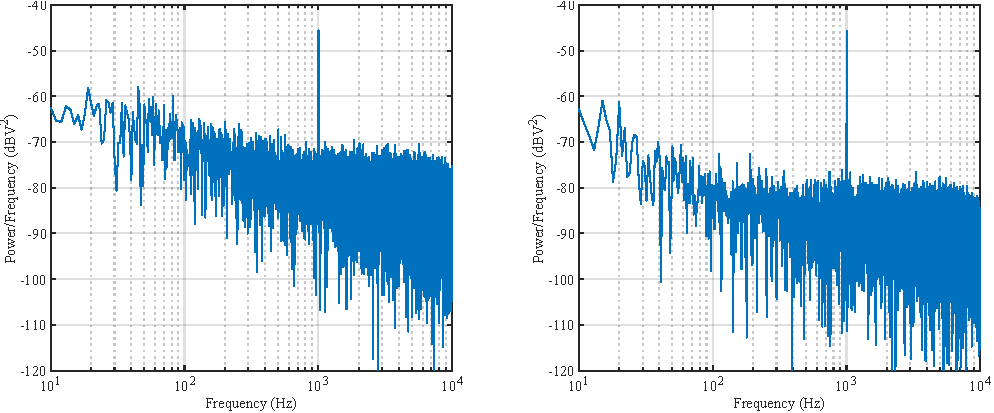
\includegraphics[width=1\linewidth]{5-Experiment/Periodogram 500mA (10mV input).pdf}}
\caption{(a) Periodogram of active optrode channel at \qty{500}{\mA} light source current with \qty{10}{\mV} peak to peak \qty{1}{\kHz} sinusoidal input signal at the active optrode (b) Periodogram of noise cancelling output channel at \qty{500}{\mA} light source current with \qty{10}{\mV} peak to peak \qty{1}{\kHz} sinusoidal input signal at the active optrode}
\label{fig_Periodogram 500mA (10mV input)}
\end{figure}

\section{Physical movement artefacts}

When mounting the nerve signal detection device on a subject, optrode systems commonly suffer artifacts due to physical movements between the system and the subject.  These artifacts are largely caused by the deformation of light fibres, and can add a significant amount of noise to the captured signals.  Since both light channel circuits are mounted in close proximity, the artifacts showing in both channels are similar.  Therefore, our active noise cancelling system is able to significantly reduce the movement-induced artifacts.  Fig.~\ref{fig_Movement Artifact} shows the result of an experiment where the light receiver board was moved while capturing data with a zero input at the active optrode.  The Active Optrode channel clearly shows substantial noise induced by movement.  Although there is still some low-frequency noise left in the Noise Cancelling Output channel, it is evident that the movement-induced noise has been largely removed.

\begin{figure}[h]
\centerline{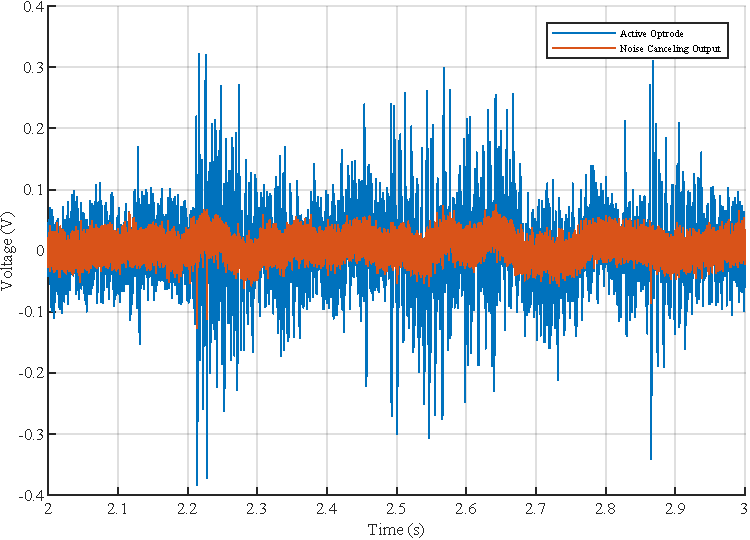
\includegraphics[scale=1]{5-Experiment/Movement Artifact.pdf}}
\caption{Movement induced artifacts and artifact removal at \qty{500}{\mA} light source current with a zero input signal to the active optrode}
\label{fig_Movement Artifact}
\end{figure}

